\documentclass{article}
\usepackage{graphicx}
\usepackage{amsmath}
\usepackage{booktabs}
\usepackage{siunitx}
\usepackage{float}

\title{Assignment 2 - EE4725 Quasi Optical Systems}
\author{Daniel Tyukov \\ Student Number: 5714699 \\ Microelectronics, TU Delft}
\date{March 2026}

\begin{document}

\maketitle

\tableofcontents
\newpage

%% ====================================================================
\section{System Parameters}
%% ====================================================================

The system under analysis is a front-fed parabolic reflector antenna with the following parameters:
\begin{itemize}
\item Operating frequency: $f = \SI{500}{GHz}$, wavelength $\lambda = \SI{0.6}{mm}$, wavenumber $k_0 = 2\pi/\lambda$
\item Feed: circular aperture of diameter $D_f = 4\lambda = \SI{2.4}{mm}$ (radius $a = 2\lambda$), with a $\hat{y}$-polarized uniform electric current distribution
\item Parabolic reflector focal length: $f = \SI{5}{m}$
\item Free-space impedance: $\zeta = 120\pi\;\Omega$
\end{itemize}

%% ====================================================================
\section{Q1: Feed Far Field (1 point)}
%% ====================================================================

The normalized far field patterns of the circular aperture feed are computed in two principal planes:
\begin{itemize}
\item \textbf{E-plane} ($\phi=90^\circ$): contains the $\hat{y}$-axis (current polarization direction)
\item \textbf{H-plane} ($\phi=0^\circ$): perpendicular to the current direction
\end{itemize}

The far field shape is governed by the Airy diffraction pattern, arising from the 2D Fourier transform of the uniform circular aperture:
\begin{equation}
\tilde{J}(k_\perp) = \pi a^2 \cdot \frac{2\,J_1(k_\perp a)}{k_\perp a}
\end{equation}
where $J_1$ is the Bessel function of the first kind and $k_\perp = k_0\sin\theta$. The first null occurs at:
\begin{equation}
\theta_{\text{null}} = \arcsin\!\left(\frac{1.22\,\lambda}{D_f}\right) = \arcsin\!\left(\frac{1.22}{4}\right) = 17.76^\circ
\end{equation}

For a $\hat{y}$-directed current, the relevant SGF column is $(G_{xy},\,G_{yy},\,G_{zy})$, and the far field is obtained via stationary phase evaluation.

\begin{figure}[H]
\centering
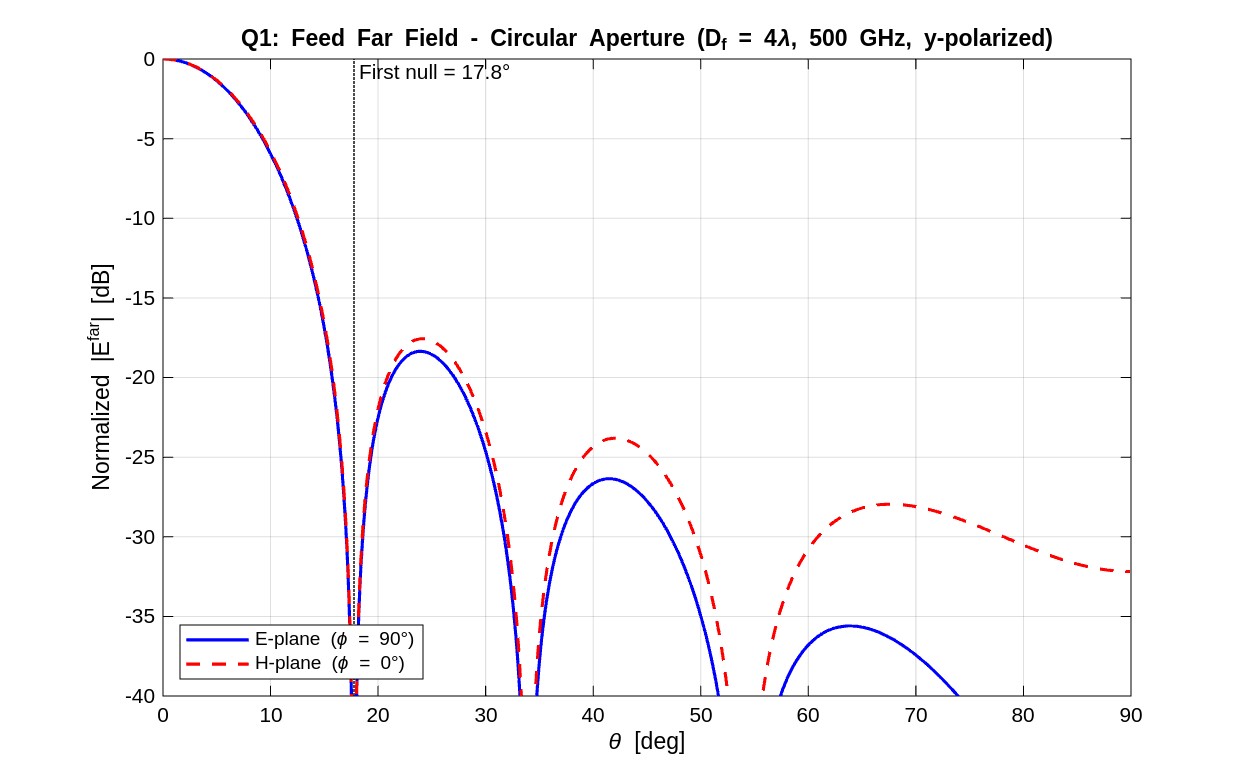
\includegraphics[width=0.85\textwidth]{figures/Q1_feed_farfield.png}
\caption{Normalized far-field pattern of the circular aperture feed ($D_f=4\lambda$, \SI{500}{GHz}, $\hat{y}$-polarized) in the E-plane and H-plane.}
\label{fig:q1}
\end{figure}

Observations from Figure~\ref{fig:q1}:
\begin{itemize}
\item The computed first null at $\theta=17.8^\circ$ matches the theoretical value of $17.76^\circ$.
\item The E-plane and H-plane patterns share the same main lobe width but differ in their sidelobe structure. In the H-plane, the SGF introduces an additional $\cos\theta$ factor on the dominant $E_\theta$ component, resulting in higher sidelobes compared to the E-plane. Conversely, the E-plane shows deeper nulls between sidelobes.
\item This E/H asymmetry is a fundamental property of linearly polarized aperture antennas: the two planes experience different projections of the vector radiation pattern.
\end{itemize}

%% ====================================================================
\section{Q2: Aperture Current Distribution, $f/D=2$ (2 points)}
%% ====================================================================

For $f/D=2$, the reflector diameter is $D=\SI{2.5}{m}$ and the half-subtended angle is:
\begin{equation}
\theta_0 = 2\arctan\!\left(\frac{D}{4f}\right) = 14.25^\circ
\end{equation}

The aperture field $\vec{E}_a$ is obtained by evaluating the feed far field at angles $(\theta',\phi')$ corresponding to each aperture point via the paraboloid mapping $\rho' = 2f\tan(\theta'/2)$, then applying the GO amplitude taper $(1+\cos\theta')/(2f)$.

The equivalent aperture currents are computed on a $201\times201$ Cartesian grid using Love's equivalence principle:
\begin{equation}
\vec{M}_s = -\hat{z}\times\vec{E}_a, \qquad \vec{J}_s = \hat{z}\times\vec{H}_a = -\frac{1}{\zeta}\vec{E}_a
\end{equation}
giving $M_x = E_{a,y}$, $M_y = -E_{a,x}$, $J_x = -E_{a,x}/\zeta$, $J_y = -E_{a,y}/\zeta$.

\begin{figure}[H]
\centering
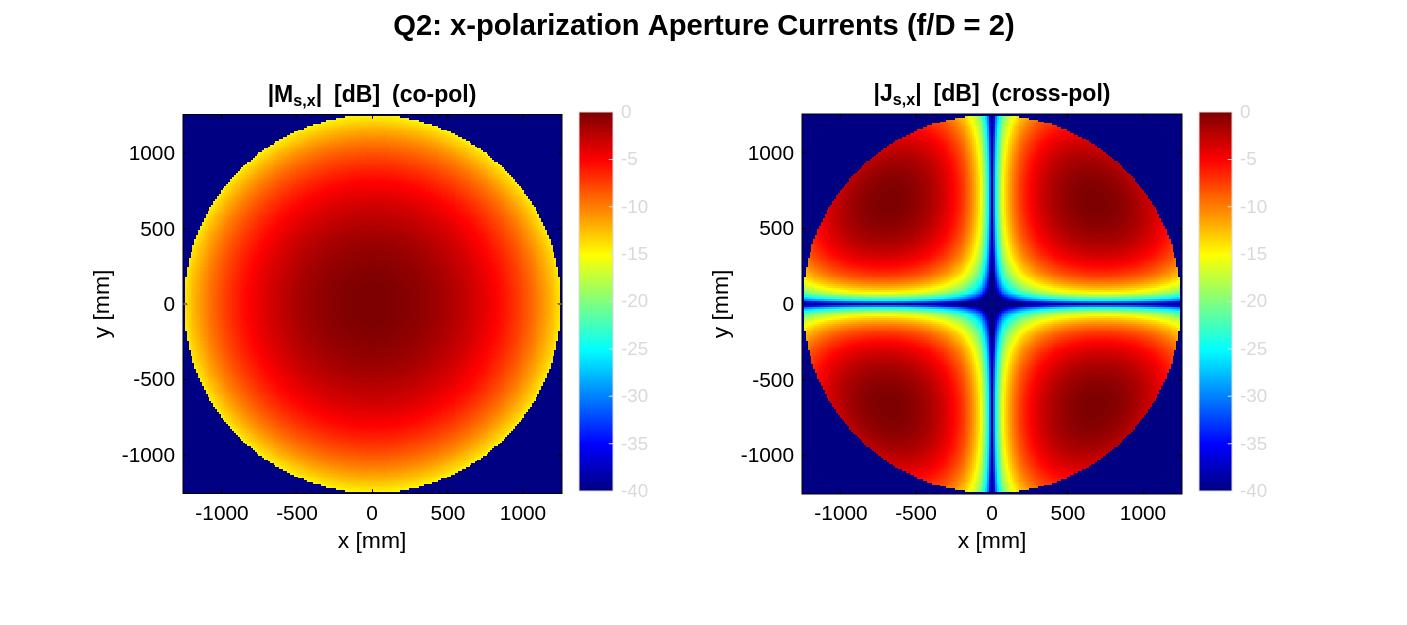
\includegraphics[width=0.85\textwidth]{figures/Q2_aperture_currents_xpol.png}
\caption{$x$-polarization aperture currents in dB: magnetic current $|M_{s,x}|$ (co-pol) and electric current $|J_{s,x}|$ (cross-pol) for $f/D=2$.}
\label{fig:q2_xpol}
\end{figure}

\begin{figure}[H]
\centering
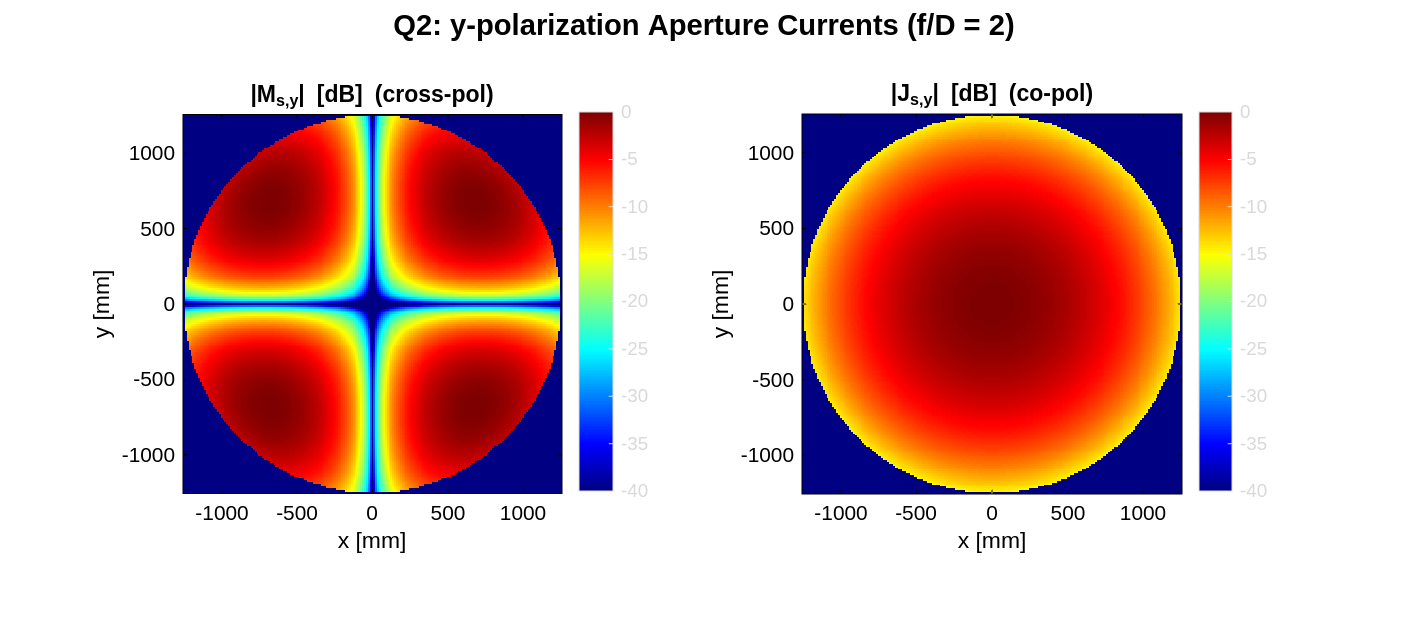
\includegraphics[width=0.85\textwidth]{figures/Q2_aperture_currents_ypol.png}
\caption{$y$-polarization aperture currents in dB: magnetic current $|M_{s,y}|$ (cross-pol) and electric current $|J_{s,y}|$ (co-pol) for $f/D=2$.}
\label{fig:q2_ypol}
\end{figure}

Observations from Figures~\ref{fig:q2_xpol} and~\ref{fig:q2_ypol}:
\begin{itemize}
\item \textbf{Co-pol components} ($M_x = E_{a,y}$ and $J_y = -E_{a,y}/\zeta$): show a smooth, nearly circularly symmetric amplitude distribution with a gradual 3--4\,dB taper from center to edge. This taper arises from the combination of the feed pattern roll-off and the GO spreading factor $(1+\cos\theta')/(2f)$.
\item \textbf{Cross-pol components} ($M_y = -E_{a,x}$ and $J_x = -E_{a,x}/\zeta$): display a characteristic quadrupolar (four-lobed) pattern with deep nulls along the $x=0$ and $y=0$ planes. The peak cross-pol level is roughly 15--20\,dB below the co-pol peak. This pattern arises from the SGF coupling between the $\hat{y}$-directed feed current and the $x$-component of the radiated field.
\end{itemize}

%% ====================================================================
\section{Q3: Reflector Far Field, $f/D=1$ (2 points)}
%% ====================================================================

For $f/D=1$, $D=\SI{5}{m}$, and $\theta_0 = 2\arctan(1/4) = 28.07^\circ$. The aperture currents are computed on a $301\times301$ grid, and the far field is obtained via numerical 2D Fourier transform using the Balanis spatial-domain formulation:
\begin{align}
E_\theta &\propto (-L_x\sin\phi + L_y\cos\phi) + \zeta\,(N_x\cos\phi + N_y\sin\phi)\cos\theta \\
E_\phi &\propto (L_x\cos\phi + L_y\sin\phi)\cos\theta + \zeta\,(N_x\sin\phi - N_y\cos\phi)
\end{align}
where $\vec{N} = \iint \vec{J}_s\,e^{j(k_x x'+k_y y')}\,dx'\,dy'$ and $\vec{L} = \iint \vec{M}_s\,e^{j(k_x x'+k_y y')}\,dx'\,dy'$.

The beam is extremely narrow: the theoretical Airy null is at $\arcsin(1.22\lambda/D) = 0.0084^\circ$ for $D=\SI{5}{m}$ at $\lambda=\SI{0.6}{mm}$.

\begin{figure}[H]
\centering
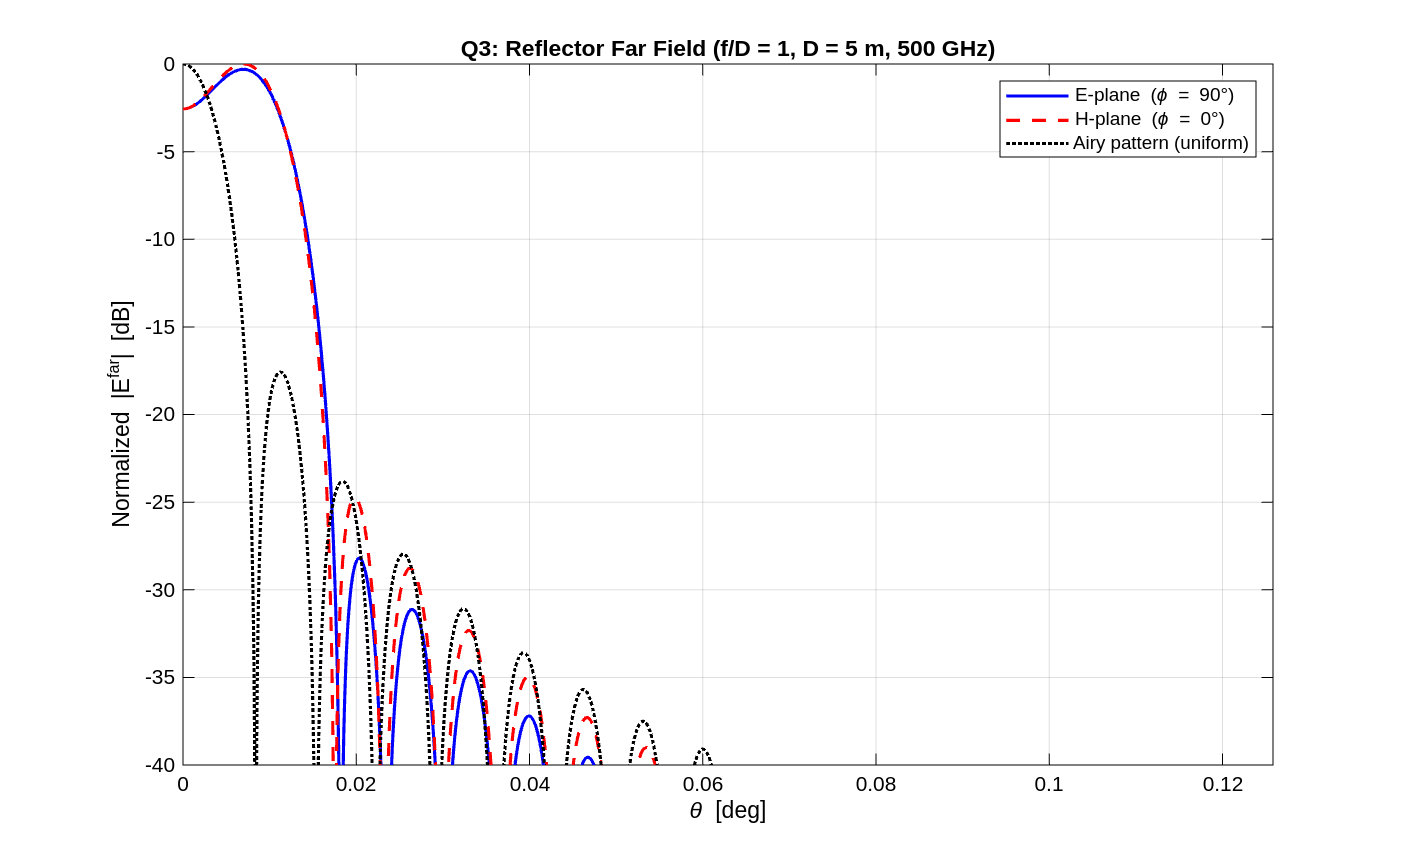
\includegraphics[width=0.85\textwidth]{figures/Q3_reflector_farfield.png}
\caption{Normalized far-field pattern of the parabolic reflector ($f/D=1$, $D=\SI{5}{m}$) in the E-plane and H-plane, compared to the Airy pattern of a uniformly illuminated aperture.}
\label{fig:q3}
\end{figure}

Observations from Figure~\ref{fig:q3}:
\begin{enumerate}
\item \textbf{Wider main beam}: The reflector pattern has its first null at approximately $0.01^\circ$, compared to $0.0084^\circ$ for the Airy pattern. This widening is due to the amplitude taper across the aperture~--- the edges are less illuminated, reducing the effective aperture size.
\item \textbf{Lower sidelobes}: The first sidelobe of the reflector pattern is approximately $-25$\,dB, significantly below the Airy pattern's first sidelobe at $-17.6$\,dB. The amplitude taper acts as a natural window function that suppresses sidelobes.
\item \textbf{E/H plane similarity}: The E-plane and H-plane patterns are very similar, with only minor differences in the sidelobe region. This is expected because the co-pol aperture distribution is nearly circularly symmetric.
\end{enumerate}

%% ====================================================================
\section{Q4: Efficiencies vs $D$ (3 points)}
%% ====================================================================

Three efficiencies are computed as a function of reflector diameter $D$ for $0.6 < f/D < 6$. The spillover efficiency is:
\begin{equation}
\eta_s = \frac{\int_0^{\theta_0}\int_0^{2\pi} U_{\text{feed}}\sin\theta'\,d\theta'\,d\phi'}{\int_0^{\pi/2}\int_0^{2\pi} U_{\text{feed}}\sin\theta'\,d\theta'\,d\phi'}
\end{equation}

The taper efficiency, using the Ludwig-3 co-pol definition $E_{\text{co}} = E_\theta\sin\phi + E_\phi\cos\phi$, is:
\begin{equation}
\eta_t = \frac{16}{\pi}\left(\frac{f}{D}\right)^2 \frac{\left|\int_0^{\theta_0}\int_0^{2\pi} |E_{\text{co}}|\,\tan\!\left(\frac{\theta'}{2}\right)\,d\theta'\,d\phi'\right|^2}{\int_0^{\theta_0}\int_0^{2\pi} G(\theta',\phi')\sin\theta'\,d\theta'\,d\phi'}
\end{equation}

The aperture efficiency is $\eta_{\text{ap}} = \eta_s\cdot\eta_t$.

\begin{figure}[H]
\centering
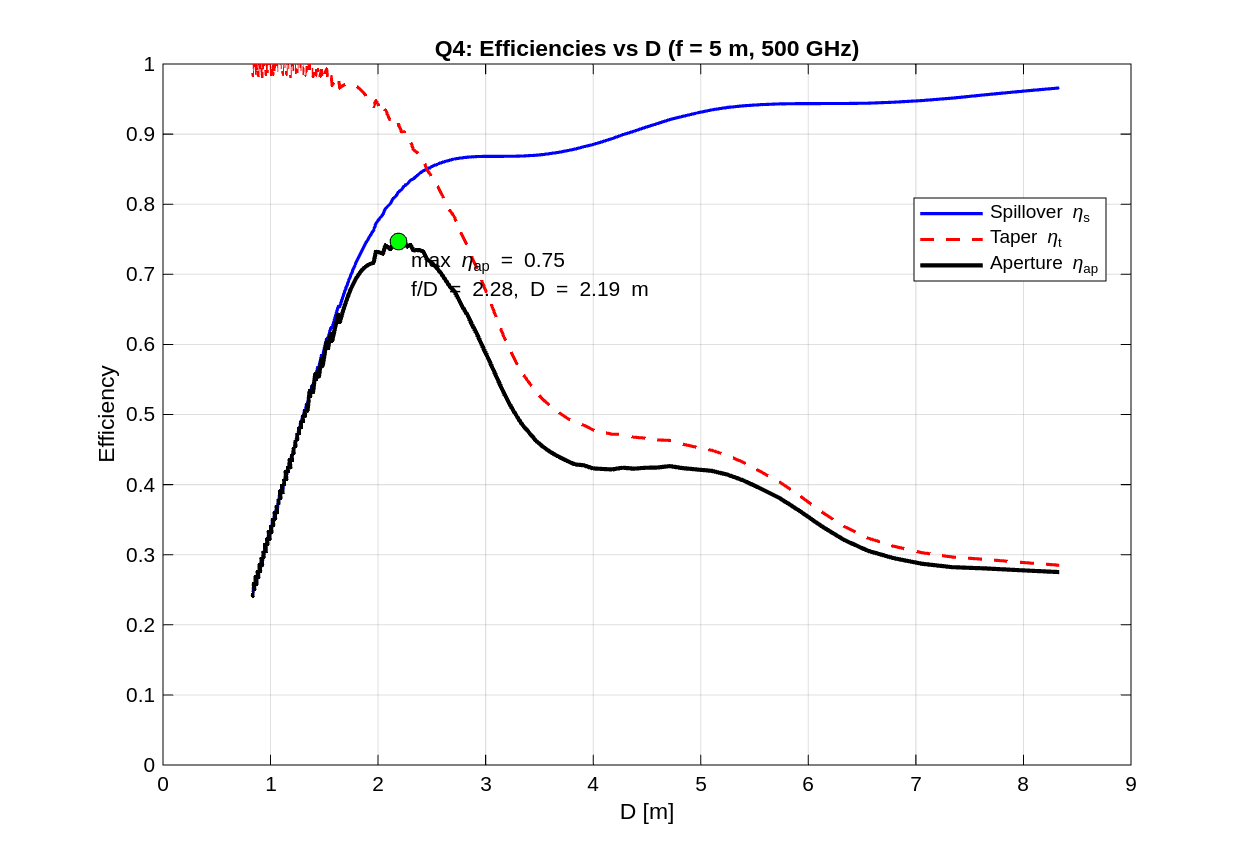
\includegraphics[width=0.85\textwidth]{figures/Q4_efficiencies.png}
\caption{Spillover, taper, and aperture efficiency vs.\ reflector diameter $D$ ($f=\SI{5}{m}$, \SI{500}{GHz}).}
\label{fig:q4}
\end{figure}

Observations from Figure~\ref{fig:q4}:
\begin{itemize}
\item \textbf{Large $D$ (small $f/D$, deep dish)}: The reflector subtends a large angle ($\theta_0$ up to ${\sim}45^\circ$ at $f/D=0.6$). Spillover efficiency $\eta_s$ is high (${\sim}0.96$) because the large dish captures most of the feed power. However, taper efficiency $\eta_t$ is poor (${\sim}0.3$) because the feed pattern has already passed through its first null at $17.8^\circ$ and the illumination is highly non-uniform.
\item \textbf{Small $D$ (large $f/D$, shallow dish)}: Taper efficiency approaches $1.0$ because only the smooth central portion of the feed pattern illuminates the dish. However, spillover efficiency drops significantly (below $0.5$ at $f/D>4$) as most feed power misses the small reflector.
\item \textbf{Optimal $D$}: The aperture efficiency peaks at $\eta_{\text{ap}} = 0.75$ at $f/D = 2.28$ ($D=\SI{2.19}{m}$), where $\eta_s = 0.87$ and $\eta_t = 0.86$. This corresponds to an edge taper of roughly $-10$ to $-12$\,dB, the well-known criterion for maximum aperture efficiency in reflector antenna design.
\end{itemize}

%% ====================================================================
\section{Q5: Directivity and Gain vs $D$ (2 points)}
%% ====================================================================

The maximum directivity, directivity, and gain are:
\begin{equation}
D_{\max} = \left(\frac{\pi D}{\lambda}\right)^2, \qquad D = \eta_t\,D_{\max}, \qquad G = \eta_s\,\eta_t\,D_{\max}
\end{equation}

\begin{figure}[H]
\centering
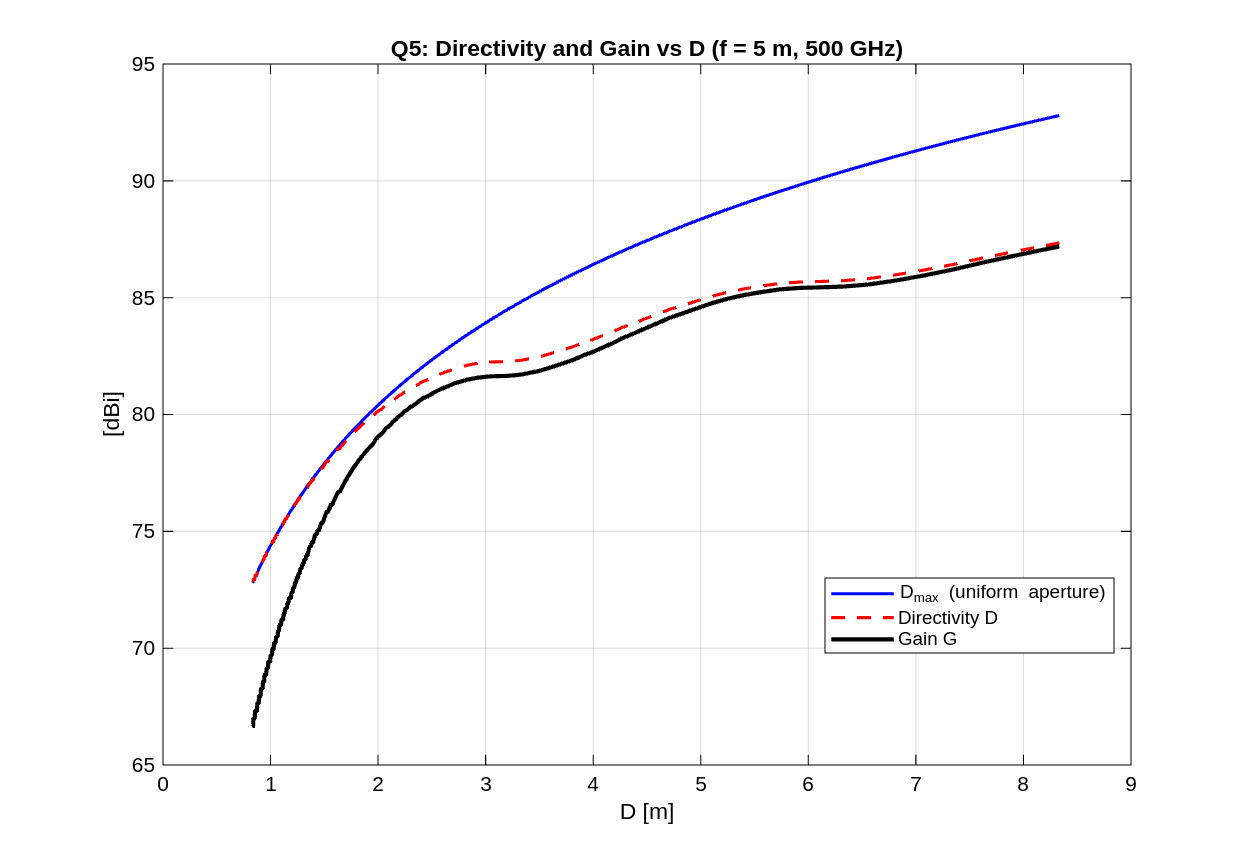
\includegraphics[width=0.85\textwidth]{figures/Q5_directivity_gain.png}
\caption{Maximum directivity $D_{\max}$, directivity $D$, and gain $G$ vs.\ reflector diameter $D$ in dBi ($f=\SI{5}{m}$, \SI{500}{GHz}).}
\label{fig:q5}
\end{figure}

Observations from Figure~\ref{fig:q5}:
\begin{itemize}
\item $D_{\max}$ increases monotonically with $D$, following the $(\pi D/\lambda)^2$ scaling. At $D=\SI{5}{m}$, $D_{\max} \approx \SI{88.4}{dBi}$. This is purely geometric~--- larger aperture means more collecting area.
\item \textbf{Directivity} $D$ is reduced from $D_{\max}$ by the taper efficiency. At large $D$ (small $f/D$), the taper loss is substantial (${\sim}$5--6\,dB) because the feed pattern illuminates the aperture very non-uniformly. At small $D$ (large $f/D$), $D$ approaches $D_{\max}$ as taper efficiency is near unity.
\item \textbf{Gain} $G$ is further reduced by spillover loss. At small $D$ (large $f/D$), the gap between $G$ and $D$ is large (up to 5+\,dB) because most feed power misses the small reflector. At large $D$ (small $f/D$), $G$ is close to $D$ since the big dish captures nearly all feed power ($\eta_s\approx 1$).
\item The relationship $G \leq D \leq D_{\max}$ always holds. The gap $D_{\max} - G$ in dB equals $-10\log_{10}(\eta_{\text{ap}})$, which is minimized at the optimal $f/D = 2.28$ where $\eta_{\text{ap}} = 0.75$ (loss of only \SI{1.25}{dB}).
\end{itemize}

\end{document}
